% =====================================================================
% Semana 3 · S3.1 — Polarización fija y punto Q
% Fundamentos de Sistemas Electrónicos Analógicos (Ingeniería Aeroespacial)
% Compilar: pdflatex semana_3_s31_polarizacion_fija.tex  (2 pasadas)
% =====================================================================
\documentclass[aspectratio=169]{beamer}

\usepackage[utf8]{inputenc}
\usepackage[T1]{fontenc}
\usepackage{lmodern}
\usepackage[spanish,es-tabla]{babel}
\usepackage{amsmath,amssymb}
\usepackage{siunitx}
\usepackage{booktabs}
\usepackage{microtype}
\usepackage{circuitikz}

\definecolor{navy}{RGB}{23,54,93}
\definecolor{navysoft}{RGB}{72,101,140}
\definecolor{gold}{RGB}{179,142,62}
\definecolor{ink}{RGB}{44,51,58}
\definecolor{soft}{RGB}{244,241,234}

\usetheme{default}
\setbeamertemplate{navigation symbols}{}
\setbeamertemplate{footline}[frame number]
\setbeamercolor{structure}{fg=navy}
\setbeamercolor{frametitle}{fg=white,bg=navy}
\setbeamercolor{title}{fg=navy}
\setbeamercolor{subtitle}{fg=navysoft}
\setbeamercolor{itemize item}{fg=gold}
\setbeamercolor{itemize subitem}{fg=gold}
\setbeamercolor{block title}{fg=white,bg=navy}
\setbeamercolor{block body}{bg=soft}
\setbeamercolor{example text}{fg=navy}
\setbeamertemplate{itemize item}{\scriptsize\raise1.25pt\hbox{\donotcoloroutermaths$\bullet$}}
\setbeamertemplate{itemize subitem}{\scriptsize\raise1.25pt\hbox{\donotcoloroutermaths$\circ$}}
\setbeamerfont{frametitle}{size=\large,series=\bfseries}

\title[S3.1 · Polarización fija]{Polarización fija y punto Q}
\subtitle{S3.1 — Simulaciones y laboratorio de la Semana 3}
\institute{Licenciatura en Ingeniería Aeroespacial\\ UNAM · ENES Unidad Juriquilla}
\author{M. en C. José de Jesús Santana Ramírez}
\date{Semestre 2027-1}

\begin{document}

% ---------------------------------------------------------------------
\begin{frame}[plain]
  \titlepage
\end{frame}

% ---------------------------------------------------------------------
\begin{frame}{Objetivos de la sesión}
  \begin{itemize}
    \item Reconocer las \textbf{regiones de operación} del TBJ: corte, activa y saturación.
    \item Calcular el \textbf{punto Q} ($I_C$, $V_{CE}$) de una polarización fija.
    \item Trazar la \textbf{recta de carga} y ubicar el punto Q.
    \item Analizar la \textbf{sensibilidad a $\beta$} de esta topología.
  \end{itemize}
  \pause
  \begin{block}{Pregunta rectora}
    Un transistor con $\beta = 100$ da un punto Q correcto. ¿Qué pasa si el lote
    siguiente trae $\beta = 200$ o si sube la temperatura?
  \end{block}
\end{frame}

% ---------------------------------------------------------------------
\begin{frame}{Teoría 1 · Regiones de operación del TBJ}
  \begin{itemize}
    \item \textbf{Corte:} $I_C \approx 0$, $V_{CE} \approx V_{CC}$ (no conduce).
    \item \textbf{Activa:} BE en directa, BC en inversa; $I_C = \beta\cdot I_B$ (zona de amplificación).
    \item \textbf{Saturación:} $I_C$ máximo, $V_{CE} \approx V_{CE(sat)} \approx 0.2\,\text{V}$ (conduce saturando).
  \end{itemize}
  \pause
  \begin{block}{Convención de signos (la de S1.2)}
    En un NPN, $I_B$ e $I_C$ \textbf{entran}, $I_E$ \textbf{sale}; $I_E = I_C + I_B \approx I_C$ si $\beta \gg 1$.
  \end{block}
\end{frame}

% ---------------------------------------------------------------------
\begin{frame}{Teoría 2 · Polarización fija}
  \begin{center}
    \resizebox{0.66\linewidth}{!}{%
    \begin{circuitikz}[american voltages, scale=1.0]
      \node[npn] (Q) at (4.2,1.6) {$Q$};
      \draw (0,0) to[V, l={$V_{CC}=12\,\mathrm{V}$}, i=$I$] (0,3.2);
      \draw (0,3.2) -- (7,3.2);
      \draw (0,0) -- (7,0);
      \node[ground] at (7,0) {};
      \draw (Q.C) to[R, l={$R_C=3.3\,\mathrm{k}$}] (7,3.2);
      \draw (Q.E) -- (4.2,0);
      \draw (Q.B) to[R, l={$R_B=470\,\mathrm{k}$}] (1.6,1.6) -- (1.6,3.2);
    \end{circuitikz}}
  \end{center}
  \[
    I_B = \frac{V_{CC}-V_{BE}}{R_B}
    \qquad
    I_C = \beta\cdot I_B
    \qquad
    V_{CE} = V_{CC} - I_C\cdot R_C
  \]
\end{frame}

% ---------------------------------------------------------------------
\begin{frame}{Ejercicio · Cálculo del punto Q}
  \begin{block}{Datos}
    \centering
    $V_{CC} = \SI{12}{\volt}$, $R_B = \SI{470}{\kilo\ohm}$, $R_C = \SI{3.3}{\kilo\ohm}$, $V_{BE} = \SI{0.7}{\volt}$, $\beta = 100$.
  \end{block}
  \begin{align*}
    I_B &= \frac{12-0.7}{470\,\text{k}\Omega} = \SI{24.0}{\micro\ampere}\\
    I_C &= 100\cdot 24.0\,\text{µA} = \boxed{\SI{2.40}{\milli\ampere}}\\
    V_{CE} &= 12 - (2.40\,\text{mA})(3.3\,\text{k}\Omega) = 12 - 7.92 = \boxed{\SI{4.08}{\volt}}
  \end{align*}
  \pause
  \begin{itemize}
    \item Punto Q: $(I_C, V_{CE}) = (2.40\,\text{mA},\,4.08\,\text{V})$, en \textbf{activa}.
    \item $V_{CE} = 0.34\cdot V_{CC}$: razonable, pero depende de $\beta$.
  \end{itemize}
\end{frame}

% ---------------------------------------------------------------------
\begin{frame}{Resultado de la simulación · Sensibilidad a $\beta$}
  \begin{center}
    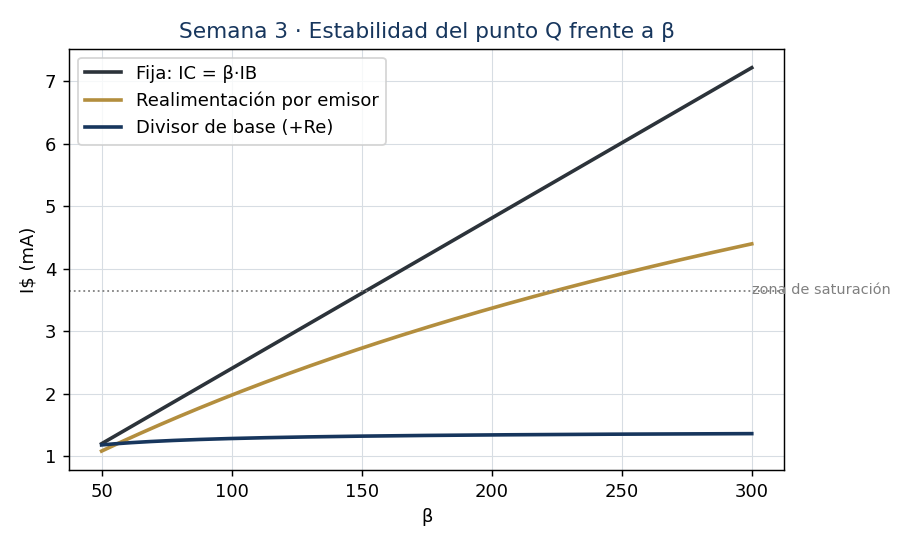
\includegraphics[width=0.72\textwidth]{figs/s3_estabilidad.png}
  \end{center}
  \begin{itemize}
    \item En la \textbf{curva gris} (fija), $I_C = \beta\cdot I_B$ crece \textbf{linealmente} con $\beta$:
      a $\beta=200$ el transistor ya \textbf{satura} (punto Q sale de activa).
    \item Es la topología \emph{menos} estable: sensible a $\beta$ y a $V_{BE}$.
  \end{itemize}
\end{frame}

% ---------------------------------------------------------------------
\begin{frame}{Errores comunes}
  \begin{table}
    \small
    \begin{tabular}{p{0.34\textwidth}p{0.30\textwidth}p{0.30\textwidth}}
      \toprule
      Error & Consecuencia & Corrección \\
      \midrule
      Usar $I_E \neq I_C$ sin justificar & Cálculo impreciso & $I_C \approx I_E$ si $\beta \gg 1$ \\
      Olvidar que $I_C$ depende de $\beta$ & Punto Q inestable & Elegir topología con RE \\
      Ignorar $V_{CE} \approx 0.2$ V en saturación & No detectar saturación & Verificar $V_{CE}$ vs $V_{CC}$ \\
      Suponer $V_{CE} = V_{CC}$ siempre & Confundir corte y activa & Calcular por la recta de carga \\
      \bottomrule
    \end{tabular}
  \end{table}
\end{frame}

% ---------------------------------------------------------------------
\begin{frame}{Preguntas de verificación}
  \begin{enumerate}
    \item ¿Qué región garantiza amplificación lineal? \uncover<2->{\emph{(Activa: $I_C = \beta I_B$.)}}
    \item Con $\beta = 200$, ¿qué pasa con el punto Q de la fija?
      \uncover<3->{\emph{($I_C = 4.8\,\text{mA}$, $V_{CE} = -3.8\,\text{V}$: satura.)}}
    \item ¿Qué es la recta de carga y dónde debe estar el Q?
    \item ¿Por qué la fija es sensible a $\beta$? \uncover<4->{\emph{($I_C = \beta I_B$.)}}
    \item ¿Qué topología usarías para un entorno variable de $-30$ a $+60\,^\circ\text{C}$?
  \end{enumerate}
\end{frame}

\end{document}
